% 2023年北京高考数学第19题解析图1：椭圆与切线/割线交点
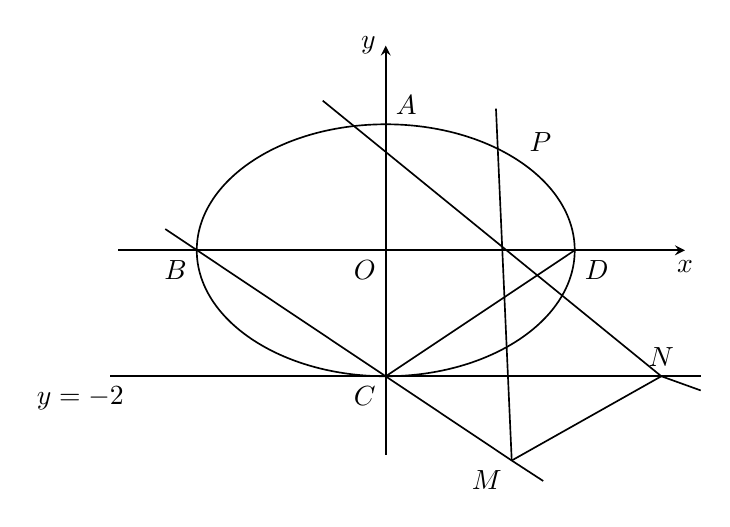
\begin{tikzpicture}[>=stealth,line width=0.6pt,font=\normalsize]
  \draw[->] (-3.4,0) -- (3.8,0) node[below] {$x$};
  \draw[->] (0,-2.6) -- (0,2.6) node[left] {$y$};
  \node[below left] at (0,0) {$O$};

  % 椭圆 x^2/9 + y^2/4 = 1, 缩放到合适大小: a=2.4, b=1.6
  \draw (0,0) ellipse (2.4 and 1.6);

  \coordinate (A) at (0,1.6);
  \coordinate (B) at (-2.4,0);
  \coordinate (C) at (0,-1.6);
  \coordinate (D) at (2.4,0);

  % 切线 y = -2
  \draw (-3.5,-1.6) -- (4.0,-1.6);
  \node[below left] at (-3.2,-1.6) {$y=-2$};

  % P 为第一象限点，取角度约 45 度
  \coordinate (P) at (1.7,1.13);

  % 直线 AP 交 y=-1.6 于 N
  % A(0,1.6), P(1.7,1.13), slope = -0.47/1.7 = -0.276
  % y - 1.6 = -0.276 x => -1.6 - 1.6 = -3.2 = -0.276 x => x_N ≈ 11.6
  % 为了绘图美观紧凑，我们绘制示意位置
  \coordinate (N) at (3.5,-1.6);
  \draw (-0.8,1.9) -- (N) -- (4.0,-1.78);

  % 直线 BC 与 直线 DP 交于 M
  \coordinate (M) at (1.6,-2.67);
  \draw (-2.8,0.27) -- (M) -- (2.0,-2.93);
  \draw (1.4,1.8) -- (M);

  % 连线 CD 与 MN
  \draw (C) -- (D);
  \draw (M) -- (N);

  % 标注
  \node[above right] at (A) {$A$};
  \node[below left] at (B) {$B$};
  \node[below left] at (C) {$C$};
  \node[below right] at (D) {$D$};
  \node[above right] at (P) {$P$};
  \node[below left] at (M) {$M$};
  \node[above] at (N) {$N$};
\end{tikzpicture}
